\section{Application of Shielding Techniques in TEM Cells}\label{sec:shielding-sim}
\subsection{ASTM ES7-83 method}\label{sec:astm-sim}
\FloatBarrier

A numerical model of a TEM cell is employed to determine the shielding effectiveness 
of barium titanate, ferrite, and silver, following the ASTM ES7-83 method described 
in \cref{sec:astm}. The electrical properties of these materials are listed in 
\autoref{tab:materials} and are chosen such that the individual contributions of high 
conductivity, lossy permeability, and lossy permittivity to the overall shielding 
performance can be investigated in isolation. Ferrite is additionally modeled with a 
magnetic loss tangent of $\tan \delta_m = 0.05$ and barium titanate with an electric 
loss tangent of $\tan \delta = 0.0095$.

The shielding material is modeled as a thin sheet of thickness $10\,\mu\text{m}$, 
positioned at the center of the TEM cell at $z = 0$. To reduce computational cost, 
the sheet is represented using impedance boundary conditions, which are valid and an 
accurate representation for this material thickness as discussed in \cref{sec:bc-shield}. 
The ASTM ES7-83 method requires the definition of a reference power to evaluate the shielding efficiency according to \eqref{eqn:SE_power}, which is set to 
$P_\mathrm{ref}=1\,\mathrm{W}$. The 
transferred power $P_\mathrm{load}$ between the TEM cell ports in the presence of the 
shielding material is then determined numerically, from which the shielding 
effectiveness as a function of frequency is computed for each material. The resulting 
shielding effectiveness are presented against frequency in \autoref{fig:se-barrium-ferrite}.

\begin{figure}[htbp]
	\centering
	\includegraphics[width=1\linewidth]{content/img/se-barrium-ferrite}
	\caption{Shielding effectiveness of a thin sheet of ferrite, barium titanate, and 
		silver as a function of frequency, determined using the ASTM ES7-83 method.}
	\label{fig:se-barrium-ferrite}
\end{figure}

\begin{table}[h]
	\centering
	{\renewcommand{\arraystretch}{1.2}
		\setlength{\tabcolsep}{12pt}
		\begin{tabular}{|l|c|c|c|}
			\hline
			Material & Rel. permittivity $\varepsilon_r$ & Rel. permeability $\mu_r$ 
			& Conductivity $\sigma$ \\
			\hline\hline
			Ferrite         & $\approx 12$    & $\approx 1{,}000$ & $0.01$\,S/m \\
			\hline
			Barium titanate & $\approx 2{,}000$ & $\approx 1$     
			& $3.64\cdot 10^{-11}$\,S/m \\
			\hline
			Silver          & $\approx 1$     & $\approx 1$       
			& $6.10\cdot 10^{7}$\,S/m \\
			\hline
	\end{tabular}}
	\caption{Electromagnetic properties of ferrite, barium titanate, and silver.}
	\label{tab:materials}
\end{table}

Silver, as a highly conductive material, exhibits a large reflection loss $R_\mathrm{dB}$ 
owing to the significant impedance mismatch between the material and the surrounding air. 
This mismatch decreases with increasing frequency, as the wave impedance of silver rises 
with frequency in accordance with \eqref{eqn:rel_wave_imp}. Simultaneously, the absorption 
coefficient $A_\mathrm{dB}$ grows with frequency, consistent with the reduction in skin 
depth at higher frequencies, as discussed in \cref{sec:skin_effect}. At low frequencies, 
the multiple-reflection correction term $B_\mathrm{dB}$ is negative and partially offsets 
the reflection loss, as discussed in \cref{sec:irt_waves}. As frequency increases, however, 
the sheet becomes electrically thicker, rendering $B_\mathrm{dB}$ negligible while the 
absorption term $A_\mathrm{dB}$ increases. Nonetheless, within the frequency range 
considered, the decrease in reflection loss is more pronounced than the increase in 
absorption, resulting in an overall reduction in shielding effectiveness with frequency.

Ferrite exhibits moderate shielding effectiveness over the investigated frequency range. 
Its high relative permeability $\mu_r$ raises the material wave impedance in accordance 
with \eqref{eqn:rel_wave_imp}, increasing the impedance mismatch with air and thus the 
reflection loss $R_\mathrm{dB}$. At low frequencies, the multiple-reflection correction 
term $B_\mathrm{dB}$ almost completely compensates the reflection loss. The absorption 
coefficient $A_\mathrm{dB}$ is limited by its low bulk conductivity $\sigma$ and magnetic 
losses parameterized by $\tan\delta_m$, so that the shielding performance is primarily 
governed by reflection.

Barium titanate, with its very high relative permittivity and near-unity permeability, 
exhibits a comparatively low wave impedance and therefore a high reflection loss 
$R_\mathrm{dB}$. Its negligible conductivity results in minimal absorption at low 
frequencies, while the multiple-reflection correction term $B_\mathrm{dB}$ almost 
completely compensates the reflection loss. As frequency increases, the growing 
electrical thickness of the sheet reduces the negative contribution of the 
multiple-reflections term $B_\mathrm{dB}$ while the dielectric loss tangent $\tan\delta$ 
gives rise to an increasing absorption contribution $A_\mathrm{dB}$, leading to a 
gradual improvement in shielding effectiveness with frequency.

\FloatBarrier
\subsection{Dual TEM cell}\label{sec:dual-tem-sim}

A simulation model of two coupled TEM cells, as shown in \autoref{fig:dual_tem_cell}, 
is constructed based on the individual cell model presented in \cref{sec:tem_cell_model}. 
The aperture separating the two cells is modeled as an empty square opening with a side 
length of $d=10\,\mathrm{mm}$, ensuring that it remains electrically small up to a 
frequency of approximately $3\,\mathrm{GHz}$. To achieve accurate results, sufficient 
mesh resolution in the aperture region is critical, as highlighted in \cref{sec:mesh}. 
Accordingly, 10 to 15 mesh elements across the aperture width are maintained throughout 
all simulations. Following the procedure outlined in \cref{sec:dual_tem_cell}, the 
electric and magnetic shielding effectiveness of ferrite, barium titanate, and silver 
are derived.

Port 1 excites the TEM cell with a constant input power of $1\,\mathrm{W}$. The sum 
$P_\mathrm{sum}$ and difference $P_\mathrm{diff}$ of the powers received at ports 3 
and 4 are then computed following \cite{Sreenivasiah_Chang_Ma_1981} as
\begin{subequations}
	\begin{equation}
		P_\mathrm{sum} = (a+b)(a+b)^*,
	\end{equation}
	\begin{equation}
		P_\mathrm{diff} = (a-b)(a-b)^*,
	\end{equation}
\end{subequations}
where $a$ and $b$ are the complex field amplitudes at ports 3 and 4, respectively. 
Evaluated for an empty aperture, these quantities serve as the reference values 
$P_\mathrm{ref,sum}$ and $P_\mathrm{ref,diff}$ required to compute the electric and 
magnetic shielding effectiveness according to \eqref{eqn:se_dual_cell_e} and 
\eqref{eqn:se_dual_cell_m}. They are shown against frequency in 
\autoref{fig:emptypowersumdiff}.

\begin{figure}[htbp]
	\centering
	\includegraphics[width=1\linewidth]{content/img/empty_power_sum_diff}
	\caption{The sum $P_\mathrm{ref,sum}$ and difference $P_\mathrm{ref,diff}$ of the 
		reference power, measured with an empty aperture and calculated with phase 
		information considered.}
	\label{fig:emptypowersumdiff}
\end{figure}

The aperture is then filled with each shielding material under investigation in turn, 
with a material thickness of $t=10\,$µm. The sum $P_\mathrm{load,sum}$ 
and difference $P_\mathrm{load,diff}$ of the powers at ports 3 and 4 are computed and 
used as the load power to derive the electric and magnetic shielding effectiveness of 
each material according to \eqref{eqn:se_dual_cell_e} and \eqref{eqn:se_dual_cell_m}. 
The derived powers for all investigated materials are shown against frequency in 
\cref{fig:powerbariumferrite,fig:powersilver}.

\begin{figure}[htbp]
	\centering
	\begin{subfigure}[b]{0.48\textwidth}
		\centering
		\includegraphics[width=1\linewidth]{content/img/power_silver}
		\caption{Silver}
		\label{fig:powersilver}
	\end{subfigure}
	\hfill
	\begin{subfigure}[b]{0.48\textwidth}
		\centering
		\includegraphics[width=1\linewidth]{content/img/power_barium_ferrite}
		\caption{Ferrite and barium titanate}
		\label{fig:powerbariumferrite}
	\end{subfigure}
	\caption{The sum $P_\mathrm{load,sum}$ and difference $P_\mathrm{load,diff}$ of 
		the output power measured at ports 3 and 4 with phase information considered.}
	\label{fig:example}
\end{figure}

The distinction between electric and magnetic shielding effectiveness is particularly 
significant in the near-field regime, where the wave impedance of the source field 
deviates substantially from the free-space impedance $\eta_0$. Electric near-field 
sources produce high-impedance fields, whereas magnetic near-field sources produce 
low-impedance fields, as mentioned in \cref{sec:irt_waves}. The shielding performance of a material depends not 
only on its electric properties but also on the degree of impedance mismatch between the 
material and the incident near-field, as expressed by \eqref{eqn:reflection_coefficient_plane_dielectric}.

Ferrite exhibits higher power transfer than barium titanate, indicating lower overall 
shielding effectiveness. For both materials, the power transfer increases with 
frequency, which can be attributed to their low bulk conductivity. Silver, by contrast, 
exhibits power transfer several orders of magnitude lower and is therefore presented 
in a separate plot for clarity. The resulting electric and magnetic shielding 
effectiveness spectra are shown in \autoref{fig:se_e_m}.

\begin{figure}[htbp]
	\centering
	\begin{subfigure}[b]{0.48\textwidth}
		\centering
		\includegraphics[width=1\linewidth]{content/img/se_silver}
		\caption{Silver}
		\label{fig:sesilver}
	\end{subfigure}
	\hfill
	\begin{subfigure}[b]{0.48\textwidth}
		\centering
		\includegraphics[width=1\linewidth]{content/img/se_barium_ferrite}
		\caption{Barium titanate and ferrite}
		\label{fig:sebariumferrite}
	\end{subfigure}
	\caption{Electric $SE_\mathrm{dB}^\mathrm{e}$ and magnetic $SE_\mathrm{dB}^\mathrm{m}$ 
		shielding effectiveness of (a) silver and (b) barium titanate and ferrite, derived 
		according to \eqref{eqn:se_dual_cell_e} and \eqref{eqn:se_dual_cell_m}.}
	\label{fig:se_e_m}
\end{figure}

Barium titanate exhibits good electric shielding characteristics but a negative 
$SE_\mathrm{dB}^\mathrm{m}$, indicating poor magnetic shielding. Negative magnetic 
shielding effectiveness values are physically possible and arise from interference 
effects at the loaded aperture, which cause the field amplitude $a$ and the received 
power at port 3 to increase \cites{4091811}[p.~63]{Jaroszewski_Thomas_Rane_2019}. 
The high relative permittivity of barium titanate lowers its material wave impedance 
(see \eqref{eqn:rel_wave_imp}), increasing the impedance mismatch with high-impedance 
electric source fields and thereby yielding a high electric shielding effectiveness. 
Conversely, this low material wave impedance reduces the mismatch with low-impedance 
magnetic near-field sources, which accounts for the poor and eventually negative 
magnetic shielding effectiveness with increasing frequency.

Ferrite, on the other hand, demonstrates a higher magnetic shielding effectiveness 
$SE_\mathrm{dB}^\mathrm{m}$ but a low or negative electric shielding effectiveness 
$SE_\mathrm{dB}^\mathrm{e}$. Its high relative permeability raises the material wave 
impedance (see \eqref{eqn:rel_wave_imp}), enhancing reflections of incident magnetic 
near-fields whose low wave impedance results in a large mismatch at the material 
surface. However, this elevated material wave impedance reduces the mismatch with 
high-impedance electric source fields, rendering ferrite a poor electric shield.

Silver demonstrates the highest overall shielding effectiveness among the materials 
investigated. Its high conductivity produces a very low material wave impedance, which 
leads to a strong impedance mismatch with electric near-field sources, 
as discussed in \cref{sec:astm-sim}. At low frequencies, the magnetic shielding 
effectiveness increases monotonically across the inspected frequency range, driven by 
the growing absorption contribution as the skin depth decreases steeply (see 
\eqref{eqn:kappa}). The electric shielding effectiveness, by contrast, begins to 
decline at higher frequencies, as the wave impedance of the material surface increases 
toward that of the high-impedance electric source field, reducing the impedance mismatch 
and the associated reflection loss $R_\mathrm{dB}$ in accordance with 
\eqref{eqn:reflection_coefficient_plane_dielectric}.
\FloatBarrier
\subsection{Antennas in shield enclosure}

Following the near-field shielding investigations, the loop and monopole antennas from 
\cref{sec:monopole,sec:loop_sim} placed inside a hollow cubic enclosure are examined, 
as shown in \cref{fig:loopantennaenclosure,fig:monopoleantennaenclosure}. The enclosure 
has a wall thickness of $10\,$µm and a side length of $6\,\text{mm}$.

\begin{figure}[htbp]
	\centering
	\begin{subfigure}[t]{0.48\textwidth}
		\centering
		\includegraphics[width=1\linewidth]{content/img/loop_antenna_enclosure}
		\caption{Loop antenna}
		\label{fig:loopantennaenclosure}
	\end{subfigure}
	\hfill
	\begin{subfigure}[t]{0.5\textwidth}
		\centering
		\raisebox{1.5mm}{\includegraphics[width=1\linewidth]{content/img/monopole_antenna_enclosure}}
		\caption{Monopole antenna}
		\label{fig:monopoleantennaenclosure}
	\end{subfigure}
	\caption{Investigated antennas placed inside a hollow cubic enclosure within the 
		TEM cell.}
	\label{fig:antennaenclosure}
\end{figure}

\autoref{fig:bariumenclosurepower} shows the radiated power from the antennas with and 
without a barium titanate enclosure. The output power of the loop antenna increases 
because the barium titanate enclosure capacitively loads the antenna, resulting in a 
reduction of the resonance frequency. This effect shifts the antenna toward a more 
efficient operating point within the investigated frequency range, as discussed in 
\cref{sec:loop_sim}. In contrast, the enclosure effectively shields the radiation of 
the monopole antenna. These results are consistent with the near-field of the monopole 
antenna being predominantly electric, as given in \eqref{eqn:compl_power_inf_elec_dipole}, 
while that of the loop antenna is predominantly magnetic, as given in \eqref{eqn:pr_loop}, 
and are in agreement with the near-field shielding investigations presented in 
\cref{sec:dual-tem-sim}.

\autoref{fig:ferriteenclosurepower} shows the corresponding radiated power for the 
ferrite enclosure. Here, the roles of the two antennas are reversed. The output power 
of the monopole antenna increases due to the ferrite enclosure inductively loading the 
antenna, while the loop antenna's radiation is attenuated.

\begin{figure}[htbp]
	\centering
	\begin{subfigure}[t]{0.48\textwidth}
		\centering
		\includegraphics[width=1\linewidth]{content/img/barium_enclosure_power}
		\caption{Barium titanate}
		\label{fig:bariumenclosurepower}
	\end{subfigure}
	\hfill
	\begin{subfigure}[t]{0.48\textwidth}
		\centering
		\includegraphics[width=1\linewidth]{content/img/ferrite_enclosure_power}
		\caption{Ferrite}
		\label{fig:ferriteenclosurepower}
	\end{subfigure}
	\caption{Radiated power as a function of frequency for the loop and monopole 
		antennas with and without enclosure.}
	\label{fig:enclosurepower}
\end{figure}

The influence of enclosure wall thickness on the radiated power is examined in 
\autoref{fig:enclosurepowervarthick}, where silver is now additionally included as a 
shielding material. As expected, increasing the wall thickness reinforces the 
shielding effects observed in \autoref{fig:enclosurepower}. Silver yields the lowest 
power transfer among all investigated materials, consistent with the high shielding 
effectiveness found and discussed in \cref{sec:dual-tem-sim,sec:astm-sim}. The output power 
of the monopole antenna within the silver enclosure increases with frequency, which 
is associated with the declining electric shielding effectiveness at higher frequencies. 
Conversely, the loop antenna produces less output power with increasing frequency, 
consistent with the monotonically increasing magnetic shielding effectiveness of silver.

\begin{figure}[htbp]
	\centering
	\begin{subfigure}[c]{0.41\textwidth}
		\centering
		\includegraphics[width=1\linewidth]{content/img/loop-shield-power}
		\caption{Loop antenna}
		\label{fig:loop-shield-power}
	\end{subfigure}
	\hfill
	\begin{subfigure}[c]{0.41\textwidth}
		\centering
		\includegraphics[width=1\linewidth]{content/img/monopole-shield-power}
		\caption{Monopole antenna}
		\label{fig:monopole-shield-power}
	\end{subfigure}
	\hfill
	\begin{subfigure}[c]{0.15\textwidth}
		\vspace{-30pt}
		\centering
		\includegraphics[width=1\linewidth]{content/img/legend-shield}
	\end{subfigure}
	\caption{Radiated power as a function of frequency for the loop and monopole 
		antennas with varying enclosure wall thickness.}
	\label{fig:enclosurepowervarthick}
\end{figure}

Additionally, resonances are observed for thick enclosures, manifesting as a 
pronounced peak in the transmitted power at approximately $2.5\,\text{GHz}$ for the 
barium titanate enclosure with a wall thickness of $100\,$µm. A similar 
trend is observed for the thickest ferrite enclosure, where the resonance frequency 
lies just outside the investigated frequency range. As shown in 
\autoref{fig:loop-resonance}, this effect corresponds to a half-wavelength resonance 
established within the enclosure cavity. The excitation of such resonant waves requires, among other things, that 
internal reflections are not fully suppressed. This proposition in turn demands that the 
multiple-reflection correction term $B_\mathrm{dB}$ remains sufficiently small in 
magnitude, as discussed in \cref{sec:irt_waves}. A larger wall thickness supports this condition by increasing the electrical 
thickness of the enclosure walls.

\begin{figure}[htbp]
	\centering
	\includegraphics[width=0.5\linewidth]{content/img/loop-resonance}
	\caption{Electric near-field distribution of the loop antenna at the resonance 
		frequency of $2.5\,\text{GHz}$, with a barium titanate shielding enclosure of 
		$100\,$µm wall thickness.}
	\label{fig:loop-resonance}
\end{figure}

\FloatBarrier
\subsection{Dipole moments in shield enclosure}
\FloatBarrier

Replacing electrically small antennas with equivalent dipole moments inside shielding 
enclosures enables of investigation of shielding performance with reduced 
computational effort. For this purpose, the equivalent dipole moments of the monopole and 
loop antennas derived in \cref{sec:eq_dip_mon,sec:eq_dip_loop} are used in place of 
the full antenna models within the enclosures depicted in \autoref{fig:antennaenclosure}. 
The radiated power produced by these dipole moments for different enclosure materials 
at a constant material thickness of $10\,$µm is shown in 
\autoref{fig:enclosurepowerdipoles}.

\begin{figure}[htbp]
	\centering
	\begin{subfigure}[c]{0.39\textwidth}
		\centering
		\includegraphics[width=1\linewidth]{content/img/dipole-shield}
		\caption{Loop antenna equivalents}
		\label{fig:loopdipoleshields}
	\end{subfigure}
	\hfill
	\begin{subfigure}[c]{0.39\textwidth}
		\centering
		\includegraphics[width=1\linewidth]{content/img/monopole_dipole_shields}
		\caption{Monopole antenna equivalents}
		\label{fig:monopoledipoleshields}
	\end{subfigure}
	\hfill
	\begin{subfigure}[c]{0.2\textwidth}
		\vspace{-30pt}
		\includegraphics[width=1\linewidth]{content/img/dipole-shield-legend}
	\end{subfigure}
	\caption{Radiated power as a function of frequency for the loop and monopole 
		antenna equivalent dipole moments in enclosures of different materials at a constant wall thickness of 10\,µm.}
	\label{fig:enclosurepowerdipoles}
\end{figure}

The dipole approximation agrees well with the full antenna model for the loop antenna 
in barium titanate and for the monopole antenna in ferrite. As the shielding 
effectiveness of the enclosure material increases relative to the respective antenna, however, the accuracy of the approximation decreases, indicating that the equivalent dipole 
moments must be adjusted accordingly to account for the interaction between the source 
and the enclosure.

\FloatBarrier
%\subsection{Shielding Antennas}
%
%\todo[inline]{shielding antennas and investigating field distribution will be done here. Some tilt in shielding material would be interesting to investigate}
%
%\subsection{Shielding Equivalent Dipole Moments}
%
%\todo[inline]{Check latex comments, which contain some good ideas. TODO Rest of section}

%\todo[inline]{Rest of shielding material section still TODO}
%\subsection{Shielding effectiveness of graphite}
%
%The reference power $P_\mathrm{ref}$ has been set to 1\,W. Using \autoref{eqn:load_power} and the S-parameters from the simulation results, $P_\mathrm{load}$ may be determined. \autoref{fig:se_graphite} demonstrates the shielding effectiveness of graphite in dB $SE_\mathrm{dB}$ over the shielding material thickness. The solution frequency is 500\,MHz. A frequency sweep shows that the reflection coefficient $S_{11}$ does not depend much on the frequency. 
%
%\begin{figure}[h]
%	\centering
%	\includegraphics[width=1\linewidth]{content/img/se_graphite.png}
%	\caption{Shielding effectiveness of graphite}
%	\label{fig:se_graphite}
%\end{figure}
%
%The components of $SE_\mathrm{dB}$ are determined according to \autoref{eqn:se_rereflections}. 
%
%\subsection{Shield effectiveness of FR4}
%
%The FR4 has a relative permittivity of $\epsilon_r=4.4$. According to \autoref{eqn:rel_wave_imp}, the relative wave impedance is $Z=0.476$. This leads to a reflection coefficient of $R=-0.355$ by \autoref{eqn:reflection_coefficient_plane_dielectric}.
%
%
%The reflection coefficient $|S_{11}|=0.045$.
%
%\subsection{Dual TEM Cell}
%
%A simulation setup of a dual TEM cell is created. A rectangular aperture with a side length of $l=5\,\mathrm{cm}$, inspired by \cite{Wilson_1981}, connects both TEM cells. One waveport 1, as in \autoref{fig:dual_tem_cell}, is excited with a power of $P=1\,\mathrm{W}$. The simulation is conducted, leaving the aperture open. A second one determines the coupling of the waveports, when the aperture is filled with a graphite sheet with a thickeness of $t=50$\,µm.
%
%At a frequency of $f=500\,\mathrm{MHz}$, the coupling between waveport 1 to the waveports 3 and 4 of the receiving TEM cell is shown in \autoref{tab:dual_tem_fwd_trans}. Only one frequency point is investigated, as the results stay roughly constant over the inspected frequency range from 100\,MHz to 1\,GHz. 
%
%
%\begin{table}
%	\centering
%	\begin{tabular}{|c|c|c|}
%		\hline
%		Forward transmission coefficient & Empty aperture & aperture filled with FR408\\\hline\hline
%		Waveport 1 to 3 $S_{13}$ & -83.80\,dB, -144.96° & -85.27\,dB, -155.79°\\\hline
%		Waveport 1 to 4 $S_{14}$ & -90.31\,dB, -144.96° & -87.14\,dB, 25.00°\\\hline
%	\end{tabular}
%	\caption{Forward transmission coefficients}
%	\label{tab:dual_tem_fwd_trans}
%\end{table}
%\todo{Why -8dB difference in empty aperture? Explained in \cite{Wilson_1981}}
%
%Using \autoref{eqn:se_dual_cell_e} and \autoref{eqn:se_dual_cell_m} leads to the shielding effectiveness for electric coupling $SE_\mathrm{dB}^\mathrm{e}=19.07\,\mathrm{dB}$ and magnetic coupling $SE_\mathrm{dB}^\mathrm{m}=-9.22\,\mathrm{dB}$. \todo{negative SE possible? Redo Simulations with finer Mesh around aperture} To get the sum $P_\mathrm{sum}$ and difference $P_\mathrm{diff}$ of powers, the phase of the signals have to be considered. With unit input power at the transmitting TEM cell, \autoref{eqn:s_param_to_power_sum} and \autoref{eqn:s_param_to_power_diff} are used for this purpose \cite{Sreenivasiah_Chang_Ma_1981}. 
%
%\begin{subequations}
%	\begin{equation}
%		P_\mathrm{sum} = (S_{13} + S_{14})(S_{13} + S_{14})^*
%		\label{eqn:s_param_to_power_sum}
%	\end{equation}
%	\begin{equation}
%		P_\mathrm{diff}= (S_{13} - S_{14})(S_{13} - S_{14})^*
%		\label{eqn:s_param_to_power_diff}
%	\end{equation}
%\end{subequations}
%
%Indicated by the phase shift of roughly 180°, the coupling between the TEM cells occur mainly due to magnetic dipoles. Due to the relative permittivity of $\epsilon _\mathrm{r}=3.66$ and the relative permeability of $\mu_r\approx 1$ of the shielding material, the magnetic fields dominate. This leads to a energy transfer mainly due to magnetic dipole moments\todo{One port receives overall more power due to the material. Is it because of the magnetic/electric dipoles in it? Check mesh around the small aperture.} The overall shielding effectiveness $SE_\mathrm{dB}=$ \autoref{eqn:dual_tem_cell_tot_power}.
%
%\begin{equation}
%	P_\mathrm{total}=|S_{13}|^2+|S_{14}|^2
%	\label{eqn:dual_tem_cell_tot_power}
%\end{equation}

% Show which dipole moments are affected by an offset in z-direction, and which ones are not.
